% Notes on writing:
% 
% * Use one sentence per line (no hard word wrapping), which makes merging different versions a lot easier.
% * Use \EM{}, \PO{} or \EA{} to add your personal comments or todos.
% * Using Git, the easiest way is probably to create your own branch and merge updates into the master branch. For Mac, see https://mac.github.com



% From DoW (603773_DOW_2013-08-05[3].pdf, p.17):
%
% D1.3) Report on LBKD model and method in the climate change domain: 
% A survey of the key publications, approaches, software and resources on Literature-Based Knowledge Discovery will be conducted. 
% In addition, any work in this area specifically related to climate change will be surveyed. 
% This will result in survey paper on LBKD in the field of climate change [month 6]


\documentclass[11pt,oneside,a4paper]{report}
\usepackage{natbib}
\usepackage{graphicx}
\usepackage{hyperref}
\usepackage{url}
\usepackage{todonotes}
% To hide all notes use 
% \usepackage[disable]{todonotes}


\newcommand{\EM}[1]{\todo[inline,author=EM,color=yellow]{#1}}
\newcommand{\PO}[1]{\todo[inline,author=PO,color=blue]{#1}}
\newcommand{\EA}[1]{\todo[inline,author=EA,color=green]{#1}}


\begin{document}

\title{Deliverable D1.1:\\ Literature-based Knowledge Discovery\\in Climate, Marine and Environmental Science}
\author{Erwin Marsi, Pinar \"Ozt\"urk, Elias Aamot}
\date{April 2014}
\maketitle

\abstract{}

\tableofcontents


\chapter{Introduction}


\chapter{Text Mining}

\todo[inline]{Describe text mining, especially entity detection, relation extraction and event extraction in BioNLP}

There is a fast growing amount of \emph{structured data} in the form of very large databases, numerical data collections, multimedia data and log files, commonly referred to as \emph{Big Data} nowadays.
Data mining, also known as \emph{knowledge discovery} from data, is about the discovery of interesting patterns in huge data collections through computational analysis.
In addition, however, there is a parallel stream of so-called \emph{unstructured data} in the form of text.
This comprises traditional sources such as newspapers, books, magazines and journals, as well as new media such webpages (Wikepedia), blogs, social media (Facebook) and messaging (Twitter).
Much of the collective knowledge of the human race is encoded in the form of text. 
Data mining methods can not handle text as input.
Therefore text needs to be converted to some form of structured data first in order to allow data mining.
This is essentialy what \emph{text mining} is about: extracting structured information from text in order to discover patterns in huge text collections through computer processing.

Text mining is applied in many different domains; for a recent overview see e.g. \citep{Aggarwal2012Mining,Weiss2012Fundamentals}.
Different domains require different approaches, techniques, tools and resources.
For example, opinion mining from social media is quite different from trend detection in financial markets. 
In this text we focus on text mining of scientfic literature to support knowledge discovery, of which literature-based discovery is a particular instance.
Text mining on scinetific literature is can be regarded as a combination of information retrieval, information extraction, natural language processing and data mining.

Information retrieval (IR) addresses the task of searching a large document collection for documents that are relevent to a user's informational needs as expressed in a search query \citep{ManningRaghavanSchutze:08}. 
The most common IR applications nowadays are web search engines which try to retrieve relevant text documents from the web, mostly webpages, on the basis of a number of keywords or phrases.
Specialized search engines exists for particular documents collections, for instance, to search scientific publications in the area of biomedicine (PUBMED).
IR is typically the first step in text mining in order to narrow down the set of relevant documents to a size managable for more in depth analysis.

Information extraction (IE) is the process of automatically extracting structured information from text \citep{Jiang2012Information}.
What type of structured information is extracted depends on the application, but usually involves two general types of information: \emph{entities} and \emph{relations}.
Entities are the things mentioned in the text.
These can be general like people, organisations, companies or places, but can also be domain-specific such as proteins, genes or drugs, organisms or anatomical parts.
Finding entities in text is called \emph{named entity recognition}.
Relations hold among pairs of entities.
For example, a company can \emph{buy} or \emph{sell} another company, a certain protein may \emph{interact} with a certain gene, or a certain drug may \emph{cause} a certain side effect.
Finding these relations in text is known as \emph{relation extraction}.  
Relations may be more complex than simple binary relations between pairs of entities.
They may involve multiple entities playing different roles, additional circumstances, or even relations between relations.
In this case, it is common to talk about \emph{events} and \emph{event extraction}.

Natural language processing (NLP) concerns automatic analysis of language by computers, usually from an applied point of view.  
Natural languages such as English or Chinese -- as opposed to artificial languages like programming languages -- are extremely complex and versatile symbolic systems that have evolved over time to enable humanes to exchange information.
Language can convey many different types of information, ranging from simple facts to complex arguments or emotional states.
Notwithstanding tremendous progress in NLP over te last decades, computers are still far from real understanding of language and currently manage a shallow understanding of meaning at best.
In practice, NLP for a specific domain, e.g. stock market reports or biomedical research articles, works significantly better than NLP for unrestricted input, because domain-specific language use and knowledge can be exploited to improve interpretation. 
Hence NLP techniques, tools and resources are often tied to a particular application domain.

Most IR systems rely to some extent on NLP.
Key word search, for instance, often involves a \emph{lemmatisation} step wich relates all morphological variants of a word to its stem.
For example, the verbs \emph{diving}, \emph{dives}, \emph{dove}, \emph{dived} are all linked to their base form \emph{dive}.
For many languages, this improves recall of relevant documents at the (slight) expense of precision.
More advanced NLP techniques are keyword expansion with automatically learned synonymns and word sense disambiguation for keywords with more than one possible interpretation.  

IE tends to be highly dependent on NLP for linguistic analysis and interpretation of the input text prior to actual extraction.
Common NLP techniques are \emph{part-of-speech tagging} (labeling tokens according to their word class such a noun, verb, preposition, etc.), lemmatisation and syntactic parsing (analysis of the grammatical structure of sentences).
The resulting linguistic annotations of the text serve as input to the algorithms for entity recognition and relation extraction, which can range from hand-written pattern matching rules to data-driven machine learning algorithms.
Like domain-specific NLP, IE is usually rather restricted in scope, that is, it targets a small subset of entities and relations of interest in the given domain, ignoring all other meaning contained in the text.    

Even with these limitations to a particular domain and to particular aspects of meaning, computers still make many mistakes in processing text, misinterpreting text and failing to detect important information.
Despite all their limitations, computers have one major advantage over humans when it comes to reading text: processing power. 
Computers can process thousands or millions of documents in a relatively short time, something a human reader would never be able to match.
The main strenght of text mining thus comes from the ability to process big text data.
One of the challenges in this area is how best to combine the fast but shallow and noisy processing capabilities of text mining systems with the slow but deep language understanding capibilities of humans.

\section{Text Mining in Biology and Medicine}

The first and most active area for research on, and application of, text mining is that of scientific publications in fields of biology and medicine, collectively referred to as \emph{biomedicine}.
One of the main reasons for this is the volume and rate of publications in biomedicine.
The MEDLINE (Medical Literature Analysis and Retrieval System Online) is a bibliographic database which indexes most biomedical publications from over 5,5000 journals since the 1950s.  
It currently contains over 21 million records and grows at a rate of approximately three publications a minute.\EM{ref}
Even though it allows researchers to retrieve documents by means of keyword search, search queries may return thousands of hits and checking all of them for relevant information is practically infeasible.
Text mining tools can offer a solution.
They can be be used for task such as further filtering of documents, clustering similar documents, automatically extracting information of interest, summarizing information through text and/or visualisation, and discovering regularities or inconsistencies.

There exist many excellent survey and review articles about text mining in biomedicine, including
\citep{Neves2012Survey,Simpson2012Biomedical,Andronis2011Literature,Ananiadou2010Event,RodriguezEsteban2009Biomedical,Zweigenbaum2009Advanced,Cohen2008Getting,Zweigenbaum2007Frontiers,Ananiadou2006,Erhardt2006Status,JenEA06,Spasic2005Text,Cohen2005Survey,Krauthammer2004Term,Blake2011Text}.
Since we do not want to duplicate these efforts with yet another survey, our discussion here is limited to a brief summary of those aspects related to literature-based knowledge discovery.  

Generic text mining tools are not well-suited for biomedical text because of highly specialized language use (jargon). 
For example, many terms have a particular meaning or do not occur at all outside of biomedical texts.
Moreover, text mining is highly dependent on the type of application, because different goals require different methods and tools.
There are a couple of prototypical applications in biomedical text mining which have driven much of the research efforts and the development of tools and resources.
One instance is finding interactions among proteins in order to find biological pathways, which are series of actions among molecules giving rise to some product or a change in a cell.
Another instance is mining interations between drugs, or between a drugs and their side effects, with the goal of drug retargetting or repurposing, that is, finding new applications for existing drugs.

entity detection

normalization

relation extraction

event extraction


\section{Machine Reading and Open Information Extraction}

\todo[inline]{NLU, open IE}

\citet{Etzioni2011Search}

\chapter{Literature-based Knowledge Discovery}

\todo[inline]{key publications, approaches, software and resources on Literature-Based Knowledge Discovery}

\todo[inline]{inference and reasoning, relation to GOFAI}

\chapter{Text mining in Climate, Marine and Environmental Science}

\todo[inline]{Text mining work in related areas, e.g. Kyoto, GeoDeepDive, text mining for Marine Ecological Genomics, environmental QA in machine reading challenge}


\section{Tools and Resources}

\subsection{Vocabularies , Taxonomies and Ontologies}

There are several specialized controlled vocabularies and ontologies which may benefit text mining in climate, marine and environmental science.
 
The Environment Ontology\footnote{\url{http://environmentontology.org/home}} (EnvO) is an ontology about environments  \citep{Buttigieg2013Environment} of biological organisms.
It provides a controlled, structured vocabulary of over 1800 terms to annotate biological entities or samples with environmental descriptors.
There are three main types of terms:

\begin{itemize}
\item \emph{biome}: e.g., boreal moist forest biome, tropical rain forest biome, and oceanic pelagic zone biome 
\item \emph{environmental feature}: e.g, mountain, pond, whale fall, and karst
\item \emph{environmental material}: e.g., sediment, soil, water, and air
\end{itemize}

\noindent The ontology is intended to facilitate integration, archiving and federated searching of environmental data.
It also contains environmental terms in the domain marine biology.
For example, Figure~\ref{fig:envo-example} shows the term \emph{marine algal bloom}.
The left side shows a definiton, known synonymyms (\emph{red tide}), and links to external definitions like the one in Wikipedia.
The right side shows a graphical representation of the ontological relations.
For instance, that \emph{marine algal bloom} is a kind of \emph{algal bloom}, which ultimately is a kind of \emph{environmental feature}, and that  \emph{marine algal bloom} is located in a\emph{ marine biome}, which ultimately is an \emph{environmental system.}

\begin{figure}
\begin{center}
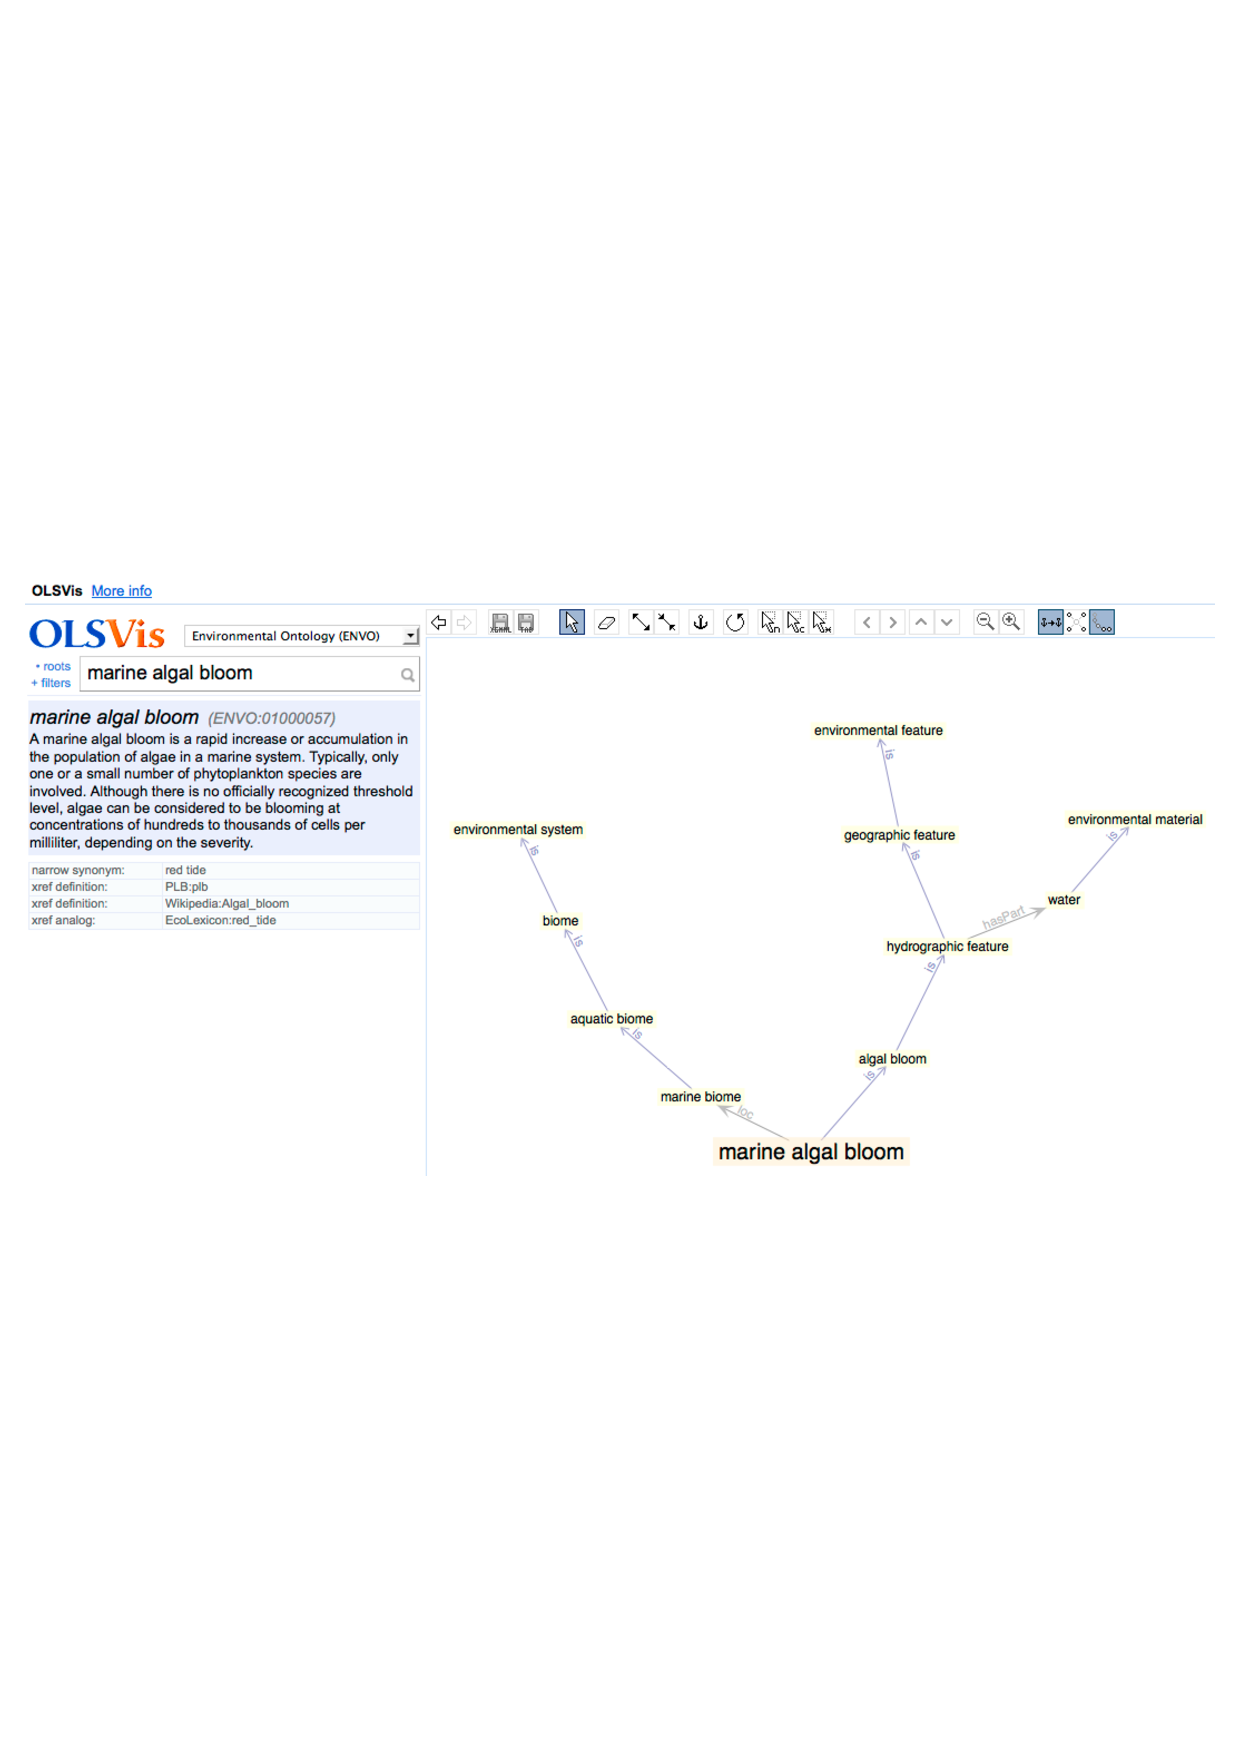
\includegraphics[scale=0.6]{envo-example.pdf}
 \caption{Example of entity \emph{marine algal bloom} in EnvO ontology}
\label{fig:envo-example}
\end{center}
\end{figure}


WoRMS\footnote{\url{http://www.marinespecies.org/}}  (World Register of Marine Species) aims to provide an authoritative and comprehensive list of names of marine organisms, including information on synonymy \citep{Costello2013Global}.
It contains over 220 thousand species, with an estmated coverage of over 95\%.
There is webservice that allows tasks such getting the full classification for your taxa, resolving unaccepted names to accepted ones or resolving a common name to a scientific name.

The Marine Metadata Interoperability\footnote{\url{https://marinemetadata.org/}} (MMI) project has as its mission promoting the exchange, integration and use of marine data through enhanced data publishing, discovery, documentation and accessibility.
It hosts. among other things, an ontology repository and associated semantic framework that can be used by the marine science community to store, manage, and work with its scientific vocabularies.


\subsection{Named Entity Taggers}

Many named entity taggers are developed for biomedicine and target specific entities of interest in this domain, such a proteins, genes and drugs.
These are of limited use for text mining in climate, marine and environmental science. 
However, there are a number of taggers for recognition and normalization of biological or chemical entities that are potentially useful for our purposes.

LINNAEUS\footnote{\url{http://linnaeus.sourceforge.net/}} is an open-source software package for species name recognition and normalization \citep{Gerner2010LINNAEUS}. 
Enities are normalized by linking them to unique indentifiers the NCBI taxonomy database\footnote{\url{http://www.ncbi.nlm.nih.gov/taxonomy}}, a curated classification and nomenclature for all of the organisms in the public sequence databases, covering about 10\% of the described species of life on the planet.
It uses a dictionary-based approach to identify species names and a set of heuristics to resolve ambiguous mentions, obtaining 94\% recall and 97\% precision on entity recognition, with 97\% of all mentions resolved to the correct NCBI taxonomy identifiers.
 
The SPECIES (Identification of Taxonomic Mentions in Text) project\footnote{\url{http://species.jensenlab.org/}} has developed taggers for species and organisms mentions in text \citep{Pafilis2013SPECIES}. 
The taggers allow for both identification of names in the text and normalization to the corresponding entries in the NCBI taxonomy.
These tools are claimed to be an order of magnitude faster than LINNAEUS.

OSCAR4\footnote{\url{https://bitbucket.org/wwmm/oscar4}} (Open Source Chemistry Analysis Routines) is an open source extensible system for the automated annotation of chemistry in scientific articles \citep{Jessop2011OSCAR4}.
It can be used to identify chemical names, reaction names, ontology terms, enzymes and chemical prefixes and adjectives, and chemical data such as state, yield, IR, NMR and mass spectra and elemental analyses. 
In addition, where possible, any chemical names detected will be annotated with structures derived either by lookup, or name-to-structure parsing using OPSIN or with identifiers from the ChEBI (Chemical Entities of Biological Interest) ontology.

ChemSpot\footnote{\url{https://www.informatik.hu-berlin.de/forschung/gebiete/wbi/resources/chemspot/chemspot/}} is another set of tools for named entity recognition and classification of chemicals in texts, including trivial names, abbreviations, molecular formulas and International Union of Pure and Applied Chemistry (IUPAC) chemical compounds. 
ChemSpot employs supervised-machine learning (Conditional Random Field) and a dictionary, as well as pattern-based recognition, a classifier model and several methods for consolidating all annotations. 
ChemSpot also performs named entity normalization by assigning identifiers from numerous chemical databases. 

CheNER\footnote{\url{http://chener.bioinfo.cnio.es/}} (Chemical Named Entity Recognizer) is another recent tool. It specializes on processing IUPAC entities, on which it is shown to outperform Chemspot \citep{Usie2014CheNER}.

The ENVIRONMENTS\footnote{\url{http://envo.her.hcmr.gr/environments.html}} (Identification of Environment Descriptive Terms in Text) project aims to produce software identifying environment descriptive terms in text, such as coral reef, cultivated land, glacier, pelagic, forest, lagoon.
It allows for orthographic variation in the way the terms are written (e.g. plural forms and spacing/hyphenation like in freshwater, fresh-water, and "fresh water).
Terms are normalized by linking them to a unique identifier is the Environmental Ontology (EnvO).
The project is ongoing and as of yet no software has been released.


\chapter{Ongoing and future work} 

\todo[inline]{Brief description of our current work and plans on LBD}

\bibliographystyle{plainnat}
\bibliography{ocwp1_d1}

\end{document}
